%!TEX root = ThesisEx.tex
% \resetdatestamp



% Don't know what these three lines are, they came with the McGill template
% \newcommand\Dfrac[2]{\frac{\displaystyle #1}{\displaystyle #2}}
% \newcommand{\mathBF}[1]{\mbox{\boldmath $#1$}}
% \newcommand{\C}[1]{\mathBF{#1}}





\chapter{Human-music listening interaction}\label{ch:human-music-listening-interaction}
\graphicspath{{./figs/ch2} }
The act of listening to music is always situated in a particular and precise context. Though being silent, still, and completely focused on music can be seen as the ideal listening situation, people are usually doing other activities when hearing music and many times choose specific music to drive or accompany these activities.
% NB: THIS INTRODUCTION SHOULD BE A BIT LONGER. IT SHOULD INTRODUCE USER- AND DATA-CENTRIC STUDIES ABOUT THE USE OF MUSIC IN EVERYDAY LIFE. THEN, IT SHOULD EXPLAIN THESE ONES.
\textcite{denora99music} extrapolated on this idea and suggested that people make use of music ``as a technology of the self'' to regulate individual emotional states and drive social agency. 
The functions of music in everyday life were studied by \textcite{sloboda01functions}. They  found that people consciously use music to modify the perception of everyday non-musical activities. Finally, \textcite{sloboda09choosing} proposed that some people develop expertise in choosing the proper music to achieve specific psychological outcomes for particular moments. However, they recognised that it is still unclear what music does to people at different times, and why they choose a particular type of music while being in a particular mood or engaged in a specific activity.
As a counterpart, Brian Whitman, co-founder and CTO of the ``music intelligence'' company The Echo Nest, and now Principal Scientist at Spotify, acknowledged that none of the music recommendation systems thus far have looked enough at the listener context \autocite{whitman13music}.
% GVM: SO WHAT? I CAN SAY THAT IT SEEMS THAT THERE IS SPACE FOR IMPROVEMENT OF MUSIC RECOMMENDERS.
% GVM: GREAT BUT OUT OF THE BLUE. WHAT ELSE I CAN SAY ABOUT THIS


In Section \ref{section:musiceveryday} of this chapter we will introduce how new technologies have changed the way in which people experience music in modern everyday life. We will also review the interactions between music, listener, and context, and the research findings about the different ways in which people make use of music.
In Section \ref{section:music-listening-studies} we will present an overview of the research methods and outcomes of studies about music preference and listening behaviour. 
The music listening factors that previous research on music preference has found relevant in the context of music preference are presented in Section \ref{section:music-listening-factors}.
These factors should provide some guidance on understanding how we listen and make use of music in our everyday lives, and therefore may be helpful for the design of better automated music recommendation systems. Music recommendations generated by these systems should be able to help people to find what they want to listen to for specific moments, matching their music listening to their everyday activities.


% Finally, in Section \ref{section:music-listening-factors} we will introduce the music listening factors that previous r{}esearch on music preference has found.
Finally, in Section \ref{sec:3-big-music-data} we will describe the characteristics and technology needed to collect and analyse large amounts of data, in Section \ref{sub:music-data-sources} we will present a review of sources of big music data, and in Section \ref{section:music_metadatabases} we will provide a comprehensive summary of all available big music listening databases. 




\section{Music in everyday life} \label{section:musiceveryday}
% \section{Psychological studies Music about music in everyday life} \label{section:musiceveryday}
Music left the spaces devoted exclusively to music enjoyment a long time ago and entered our daily life, surrounding and accompanying us wherever we go. These days, it is possible to listen to music by means of headphones or loudspeakers in just about any setting.
Moreover, fast technological changes in the last two decades have led to changes in the availability and diversity of music at one's disposal as well as in the ways in which we enjoy, use, and ``consume'' music. In particular, the digital revolution and the miniaturization and portability of new music playback equipment have made music ubiquitous in everyday life. People now can listen to practically any music at any time by means of carrying their own music collections in portable devices or by accessing massive online repositories of music. 

The thoughts about experiencing music in everyday life posed by \textcite[p. 499]{konecni82social} more than 30 years ago seem valid, contemporary, and omnipresent: 

\begin{quote}
% \onehalfspacing% <--- Local line spacing
``... one of the most important ... changes in music appreciation is the fact that music is nowadays so frequently enjoyed in a great variety of social contexts ... active listening to music has become fully embedded in the stream of daily life ... People listen to music while working, talking, eating, engaging in sexual intercourse ... What music does to people at different times, why they choose to listen to it so much, and why they choose a particular type of music while engages in a particular activity---all of these are important and unanswered questions.''
\end{quote}

\textcite{konecni82social} emphasised that listeners are stimulated not only by the arousal potential of the music but also by their immediate environment. As a result, they sum up the arousal from the music and from the listening context where the music is experienced. People within environments with high levels of arousal choose low-arousal music to moderate the excess of arousal of the listening context, and vice versa. 
Although this model can be seen as a continuous interaction between music and the listening context. However, it does not account for the fact that people sometimes want to polarise or perpetuate, instead of moderate, their levels of arousal when choosing music. 
For example, polarisation approaches can be observed in situations such as dancing with friends at parties, or when singing or listening to soft music at a child's bedtime.

Based on \citeauthor{konecni82social}'s model, \citeauthor{north96situational} developed a series of experiments in order to try to understand people's preferences and choices of music in everyday life.
In \textcite{north96situational}, they asked a group of young people to rate the likeness of a set of verbal descriptions with a set of everyday life listening situations. They found that the preferences of listeners varied with the listening environment, but this pattern did not follow strictly a pattern of arousal moderation. It seemed that this group of people sometimes chose music to perpetuate a state.
Later on, they asked people to choose music for accompanying physical exercise, for relaxation, and also for listening to music \textit{after} those activities \autocite{north00musical}.  They found that individuals engaged in activities usually wanted to maintain their levels of arousal, but following the activity, they wanted to change those levels. As a result, they hypothesised that the musical preferences of people depended upon their goals, and what they called arousal-based goals.

\citeauthor{north08musical} also studied other characteristics that may influence people's perception of and preference for music.
They noted that people change the preferences for music pieces they express depending upon who else is listening to, or has expressed liking for, the same music pieces. The authors called this characteristic compliance effects \autocite{north08musical}. % Crowther (1985)
Moreover, they also used the concept of prestige for denoting the change in the expressed preferences of listeners for music that they are not particularly familiar with, but that they think belong to a particular social group, as in the case of most academic music \autocite{north07lifestyle}. 
These two characteristics are consistent with the thoughts of \textcite{bourdieu84distinction}, who studied the aesthetic preferences and taste of people for cultural objects and found that these are rooted in the social structure. That is, in people's education and in the social classes that they are part of.
% Moreover, Furman and Duke (1988)

\textcite{hargreaves05how} developed a conceptual model designed to explain the interactions between music, listener, and listening situation. They named their model the reciprocal response model.
In this model, the effects between the three factors are bi-directional and any of the factors affect the other two in a  reciprocal feedback fashion.
Hence, music and listener are not the only factors in the interaction between music and listener; the context of listening is a third variable that influences, and is influenced by, the two others. 

The reciprocal response model establishes that the relationship between music and listening context refers to the idea that some music genres and styles fit better for certain places or activities. 
The relationship between listening situation and listener refers to the existence of different individual uses of music to achieve particular goals for specific contexts. 
Finally, the relationship between listener and music establishes the constant evolution and change in individual preferences and taste. Consequently, music is experienced by listeners within specific listening contexts or situations that modulate people's perception about it.

People use music in different ways and so understanding these uses has also been a topic of research. \textcite{sloboda09choosing} identified an array of different recurring functions when people choose music for accompanying activities with non-musical goals. They found that music is used as distraction to reduce boredom, or as a means of energizing and maintaining task attention and arousal. It is also used as entrainment when performing repetitive tasks that may need synchronizing one's movements with rhythmic pulses in the music, or as a meaning enhancer to activities, by adding an external value and changing our perception of them.
However, when the activities people perform are related to focused music listening, \citeauthor{sloboda09choosing} alluded to other different uses. These were reminiscence, or the reminding oneself of past events; mood management, or using music to modulate our emotions; and using music as a confirmation of social identity, when we use it to carry messages to others about ourselves.


% \section{Techniques to characterize people's use of music in everyday life}
\section{Music listening studies}\label{section:music-listening-studies}
Investigating how people listen to music and how they make use of music in everyday life can be done through a number of means.
Previous research, especially coming from the music psychology field, usually implemented \emph{user-driven} studies. In this type of studies all the data collection comes directly from asking, interviewing, or observing people. 
An alternative method is the \emph{data-driven} approach, where large amounts of data collected from people's digital traces is used to try to understand how people listen to and use music. These two approaches are complementary. While user-driven studies are designed to collect data about specific research questions, they are expensive to run, their coverage is limited, and subjects must agree to participate in the study. As a result, the population sample is usually biased, especially towards freshmen psychology undergraduate students from a specific university, and so studies carried out with these methods may not reflect the everyday listening practices of a broad population. 
On the other hand, data-driven studies make use of big datasets of music listening or music preference logs to analyse a much larger population with lower costs of implementation, with data point that usually cover longer periods of time. 
% and, perhaps paradoxically, more ecological validity since people are not necessarily aware of being part of a study.
Typically, however, data-driven studies are based on datasets that were not necessarily designed to answer a specific set of research questions. As a result, in these type of studies researchers have to find a way of filtering, parsing, and aggregating the data in order to try to to answer their research questions.

In the next two subsections we will provide a review of some user-driven and data-driven studies on music listening behaviour in terms of their methods and results.

\subsection{User-driven studies}
A great portion of data and evidence in relation to the uses of music in everyday life comes from music psychology research using qualitative ethnographic methods. We will now review previous studies and findings about people's use of music using these methods.

\begin{description}
	\item[Free questionnaires and interviews] The logic and motivation behind music listening be\-haviours are too complex to be captured with simple questionnaires. As a result, researchers have used free questionnaires and interviews to make listeners freely talk about how they make use of music in their everyday life. 
	\textcite{north96situational} wanted to understand the interaction and influence between the listening situation on reported musical preferences. By means of questionnaires, their study found that participants' reported musical preference varied between the proposed listening situations. Their research only considered undergraduate students of the same university, and so their conclusions may be biased towards only understanding the preferences of a particular group of people, with probably similar  taste, experiences, and exposure to music. 
	Later on, \textcite{denora00music} interviewed a group of 52 women from the United States and United Kingdom aged 18 to 77 about their uses and choices of music in everyday contexts.
	The interviewees described how they use music for different goals, stating that the choice of music depended upon the requirements of the activity they were doing, as well as in how they recall using the same music in the past.
	With the goal of understanding people's music preferences and listening behaviour throughout the day, but focused on what those people perceived as important in shaping their music preferences, \textcite{greasley06music} interviewed 23 British young adults and adults in their own homes.
	They found that listeners were consciously aware about their use of music as a mood regulation agent, and also that people's preferences can not be simply categorised in terms of musical genres. 
	\textcite{chamorro-premuzic07personality} conducted a questionnaire-based study on 341 people to understand the correlation between individual traits and specific uses of music in everyday life. They found that differences in cognitive ability and personality traits influence how people make use of music in everyday life. Their study, however, was limited to undergraduate students from the US and UK.

	\item[Surveys] This method has been extensively used to study large but limited populations about how they make use of music in their everyday lives. \textcite{north00importance} surveyed a few thousand British adolescents about the reasons why they listened to music. The authors found that music was of central importance for adolescents. It helped them to fulfil their emotional and cognitive needs as well as to project an image of themselves to other people. 
	\textcite{haake06music} surveyed the use and effects of music in working environments, particularly offices, and found that self-selected music was perceived as enhancing personal well-being as well as work performance. 
	However, their study did not provide any insights about people's perception on music that they listened but did not choose, which is a common listening situation in shared working spaces.
    Surveys were also used to understand how people use music while driving \autocite{dibben07exploratory} and to understand how chronic pain sufferers use music as pain management \autocite{mitchell07survey}. Findings of these studies show that music is used by people in those contexts and conditions with different function goals, such as distraction, energisation, and meaning enhancement.


	\item[Simulated environments] Studying how people select and use music in everyday life situation requires ecological validity (i.e., a real-life situational context). However, some studies have been carried out in laboratories and simulated environments, where it is easier to isolate the factors to measure, and where the many variables of every day life contexts can be controlled. 
	For example, \textcite{north00musical} designed an experimental setting to try to understanding how people make use of music in order to maintain, or change, a state of arousal. They exposed listeners in a soundproof laboratory to specially composed music and sounds while they were doing exercising and relaxing activities. They found that listeners tended to prefer music to achieve arousal-based goals, and that musical preferences vary with the listening situation and activity. 
	This type of study has also been used to test the effects of different musical features in people's perception on music. For example, \textcite{beh99performance} and \textcite{brodsky01effects} studied the relation of the amplitude levels of music and the effects of musical tempi, respectively, with the performance and behaviour of people while driving. Participants were studied using simulated conditions since the task at hand may be dangerous. The results showed that there is a correlation between the intensity of music and the vigilance performance and also between the tempo of background music and the participants' perceived speed. Their results, however, require further investigation since those studies did not replicate real-life driving conditions and may affect participants' responses. Also, the population of the study was again biased towards university undergraduate students.

	
	\item[Mass observation] Studies based on the anonymous observation of people's behaviour in real-life contexts have been also used to understand their reaction to music. This technique was used by \textcite{denora00music} to investigate entrainment in relation to music and exercise by means of observing weekly aerobic sessions over a one-year lapse. She also analysed people's behaviour in music therapy sessions, karaoke evenings, and by studying the use of music in the retail sector. \textcite{cunningham03ethnographic} observed people's behaviour in public spaces, such as music shops and the music section of libraries, to understand how people searched and browsed for music in real-life environments. After the observations, the authors approached people using interviews and focus groups in order to complement and provide contextual information to their study.

	\item[Experience sampling method (ESM)] ESM has been used in music listening research to study what people are actually experiencing in terms of music throughout the whole day at different levels of granularity. When participating in an ESM experiment, people are asked to stop at non pre-specified times of the day, over several days, and are required to take notes right away about their listening context and experience.  By using this approach, participants provide information while they are in a specific listening setting, overcoming the problem of recalling experiences retrospectively. Therefore, ESM allows researchers to collect details about music listening in the many possible contexts in which people experience it. 
	\textcite{sloboda01functions} used ESM to address how people's moods change as a consequence of hearing music. They found that when personal choice over the music was involved, people were more positive, alert, and focused in the present. Although they noticed people were highly exposed to music during their daily life, just a few episodes involved listening to music exclusively. In other words, music tended to be used as an accompaniment to other activities. 
	\textcite{north04uses} also employed ESM to collect data about with whom participants were listened to music, what they were listening to, and where they were listening, using forced-choice response. This study was much larger in scope and  population size than the one by \citeauthor{sloboda01functions}, but their results were similar in regard to the attitude of the participants toward music heard in everyday life. In other words, music was rarely the participant's main focus, it was used as means to achieve other goals. In addition, it was found that the value assigned to music depended upon the listening situation and the social context.
    \textcite{greasley11exploring} also designed an ESM study in order to study the engagement with music in everyday life, but they designed the ESM study with forced-choice as well open-ended responses and performed post-study interviews in order to collect qualitative data. They corroborated previous findings on musical preferences and uses of music but also realised some of the flaws of using ESM, such as not accounting for intra-individual factors which may affect the way in which people respond to and use music, and the lack of accounting for participants' previous experiences with music due to the short sampling period.
\end{description}

In contrast to user-driven studies, data-driven studies can take advantage of a stream of data that is constantly generated and submitted by listeners to databases or web based services. 
% Since the Web 2.0, the number of music services that offer web-based access has increased enormously  
In the next sections, we will provide details about this kind of study, review previous research that takes this approach, and summarize insights gained from previous research on factors affecting preferences in music listening.


\subsection{Data-driven studies} \label{sub:data-driven studies}
Data-driven methods require the analysis of large amounts of user data.
Some of the general terms used to denote this methodology and related techniques are lifelogging, life tracking, quantified self, and personal informatics \autocite{baur11thesis}. 
In the case of music, data can be gathered by collecting the interactions between listeners and online digital music services, for example.
Processes of filtering, selection, aggregation, and abstraction of the data are subsequently required to test hypotheses or infer conclusions about people's listening history, behaviour, or their use of music in everyday life settings. 


Advantages of using usage log data are: 
(i) the scale, because it is not a limiting factor as in user-driven studies; 
(ii) statistical power to infer conclusions, due to their large sample size; 
(iii) wide demographic and geographic representation, because they can collect worldwide data from a large sample of the population by means of web-based environments; 
(iv) ability measure people's preferences over extended time of the study, since listening data can be collected over long periods; and finally, 
(v) improved ecological validity since the data can be collected without directly interfering with users \autocite{rijke12logfileanalysis}. 
This last advantage is questionable, since generally only computer-savvy listeners are reached with these studies, but this trend is changing rapidly. Common downsides of data-driven music studies are the fact that generally  the data only represent a part of the daily experiences of people with music, and the sample size can be large enough to infer conclusions that work at a big scale, but not necessarily on a smaller scale. As a result, conclusions using these methods need to be carefully drawn. 



Gathering music listening logs can be achieved by collecting data from several social media and online music services. \textcite{baur11thesis} categorised two types of collecting systems: local collectors, which record music logs within their own framework (e.g., Apple's iTunes and iPod); and global collectors, which collect and aggregate music log data from several sources. 
Not every service that gathers listening logs allows for public access to those logs, but a few of them allow the free use of the data for academic research or non-commercial use. Currently, music services that offer their data are Last.fm,\footnote{The Last.fm service is available at \url{http://www.last.fm}} Libre.fm,\footnote{The community-driven music service Libre.fm is available at \url{https://libre.fm/}} and ListenBrainz.\footnote{The ListenBrainz project is available at \url{https://listenbrainz.org/}} The latter is a spin-off of the MetaBrainz Foundation with the goal of offering public and permanent store for listeners' listening data. The service allows listeners to upload data dumps of listening histories from Last.fm into its database, and makes the data available under a CC0 license, which means its is in the public domain.



Music listening log data have been used in many data-driven studies for studying people's listening behaviour and music preference. 
\textcite{shin09contextaware} studied the use of raw user-context information to improve the performance of a music recommendation model. In order to achieve this, they collected usage log data from a music streaming service and inferred a temporal listening context from the logs. Although they reported a recommendation accuracy increase when using the contextual data it is not clear how they extracted raw context since the music logs did not provide specific information about the time zone where they were generated. 

\textcite{baltrunas09towards} collected and analysed the listening histories of about three hundred listeners, and tried to infer commonalities in patterns of musical consumption. By aggregating the listening data into several different daily and weekly segments, and inferring the implicit preferences of listeners from their ranking artists and track, the authors were able to improve the accuracy of a music recommendation model by three percent.


\textcite{park10temporal} analysed the temporal dynamics of one-year usage log data from several thousands of Korean users of a large online digital music service. They studied the temporal periodicities of listening behaviour in terms of exposure to music and preference for music genres. Although they found statistically significant hourly and daily differences in listening events, they did not find significant trends on the preference for music genres.

Using four-year data for about 500 users of a music streaming service, \textcite{herrera10rocking} modelled the listeners' genre and artist preferences during different times of the day and days of the week. The authors only analysed the interactions between listeners and their top listened artists and musical genres per user. Even with this small subset, they found that only a small percentage of the listeners tended to prefer certain artists and genres at specific moments of the day and at certain days of the week. 

\textcite{baur12listening} studied the temporal characteristics and user's personality traits of 310 users of a music streaming service by means of performing principal components analysis on music listening logs spanning up to six years. They searched for correlations between demographic, behavioural, seasonal, and temporal dimensions between listeners in the dataset and the music items they experienced. The authors found a set of 13 components that explained 75 percent of the variance in the music preference data. 
% Since their approach was based on principal component analysis there was no mathematical formulation for the components and there was no explanation about how they conceptualised them. 
In particular, their analysis showed the impact of seasons and the interest of listeners in variety when choosing music. It is not clear how they were able to isolate seasons since the data they collected did not provide this information. Also, there is no mathematical formulation for how they correlate the variability in music listening events and one of the components of their analysis.

\textcite{teixeira12towards} analysed the listening history of 4K users of an online digital music service living in a single time zone. The author tried to characterise their music listening sessions by analysing the musical genres they listened to with respect to time and session. However, he was not able to validate any rules because of the large variability in people's listening preferences.






As we have seen above, user-driven and data-driven techniques for studying people's use of music and listening behaviour in everyday life provide different ways of approaching the research. 
While some user-driven studies are designed to collect quantitative data to test specific questions and hypotheses, others are more qualitative in design, and so they collect free, open responses to fully capture the richness and complexity of responses to music in everyday life. 
Data-driven studies, on the other hand, usually gather data from large databases of music listening logs for which users have already agreed to the possibility of sharing their behavioural data.
Then, statistical and machine learning techniques are trained with the collected data in order to perform classification or prediction tasks.  
In the next subsection we will provide an overview of the research findings in some of the music listening factors that affect people's music preferences in everyday life.


\section{Music listening factors}\label{section:music-listening-factors}
How people make use of music their everyday lives is a complex topic. 
Each person uses music in a different way, but a single person can also use it differently on a daily basis, because the same piece of music can have a different meaning for different people, and this meaning can depend upon the activities and the context the listener is in.
Therefore, creating a single model to describe every interaction is incredibly difficult, if not impossible. 
However, previous findings in the literature may be helpful to understand the relation between how people choose and use music in their everyday life experiences, and the different listening factors that impact their choices. 
Now we will describe some of these findings in relation to personal, social, demographic, and temporal dimensions.


% ``At the level of daily life, music has power. It is implicated in every dimension of social agency (DeNora, 2000, 2003). Music may influence how people compose their bodies, how they feel---in terms of energy and emotion---about themselves, about others, and about situations. Music may imply and, in some cases, elicit modes of conduct. To be in control of the soundtrack of social action is to provide a framework for the organization of social agency, a framework for how people perceive (consciously or subconsciously) potential avenues of conduct and thus potential for learning self-care, health and well-being, e.g. how to use music---what music does, what it can do and how it can be tapped for social purposes. Perhaps this participatory CD design, then, is one way in which to create informal ``health promoting'' cultures of learning, increasing practical (active) musicking involvement for the majority of local communities.''\shortcite{batt05music}


\begin{description}

\item[Personality] Music plays an incredibly large role in many aspects of people's social lives. It can influence how people feel about themselves, about others, and even about certain situations. 
The relation of people's personality and music preference has been mainly studied by means of user-driven studies.
By means of open interviews, \textcite{denora00music} found that people use music as a way to organise their internal and surrounding social worlds. In other words, people know what music they have to listen to in determined contexts in order to obtain certain goals. 
Later on, \textcite{denora01aesthetic} suggested that in this sense, people behave as their own disc jockey. 

In terms of the relation between personality traits and listening styles, and by means of doing latent factor analysis in a large sample of undergraduate students, \textcite{rentfrow03doremi} found that there were correlations between music preferences, personality dimensions, self-views, and cognitive abilities of the group of people under study. 
Based on, and expanding on, those findings, \textcite{chamorro-premuzic07personality} compared IQ scores of listeners with their listening strategies, and also found correlations between young people's personality traits and their music using habits. \textcite{north08musical} found that the two main approaches used by people when choosing music, in terms of their personality are: (i) people compensate for aspects of their personality when choosing specific music pieces, and (ii)  people opt for certain music to reflect and exacerbate aspects of their personality. 
Their finding suggests that people are consciously or unconsciously using music to signal something to others about their personality and to alter how others perceive them.

\item[Social context] How the social context modulates people's preference on music has been widely investigated. By means of a series of user-driven studies, \textcite{kemp96musical, north96situational} found that people use music to achieve particular goals that depend upon the activities they are doing and the context where they are immersed. 
Musical preferences are thus associated with the listening environment of the musical experience. 
Furthermore, \textcite{north04uses} found that a listener's affinity for music depends upon who the listener is with, where the listeners are, and whether they have chosen to hear the music or not. 
Expanding on this, \textcite{rana07role} used ESM to study the daily life experiences of Pakistani listeners, and found that the greatest number of listening episodes occurred in the presence of other people.
These studies also showed that music is usually experienced during the course of other activities, generally as background to those activities. \textcite{denora00music}, however, inferred from her series of interviews that people use music to continually reconstruct the aims and goals of their activities, instead of only using it as background. In other words, people use music as a ``process'' rather than as an ``object.''

\item[Gender] \textcite{baur11thesis} found that there are no statistically significant differences in how males and females act in terms of their musical preferences and behaviour.
However, in terms of the types of music people choose to listen to, by means of gathering listener histories only for  Dutch users from a music streaming service, \textcite{berkers10gendered} found that males and females had the same preferred artists (Coldplay and Radiohead), both listened primarily to male artists, and both had a similar range of genres they listened to. However, when he examined beyond people's top preferred artists, he found that young females listened more often to ``softer,'' and more mainstream music genres, they listened to more female artists, and they listened to a wider range of genres than males. 
Similar trends were observed by \textcite{north08musical}, who also found that femamles, in general, prefer ``softer'' musical styles (e.g., mainstream pop and R\&B) and males prefer ``harder'' and more aggressive styles (e.g., rock and rap). 
Findings by \textcite{millar08selective} went further. By means of questionnaires to an Australian population of young people, they studied gender differences in artist preferences and concluded that there was a strong gender bias in the majority of males towards listening mainly to male musicians.
In terms of the functions that people assign to music, \textcite{north00importance} found that young females and males use music differently. While females use it as a way of fulfilling their emotional needs (i.e., as mood optimisation), young males use music to cause an impression on other people (i.e., as impression management).


\item[Age] Research findings about the relation of age and music have established that younger people change their musical taste radically and regularly \autocite{hargreaves95effects}, but they settle for a more general open listening style and stabilise their music preferences in their late adolescence or early adulthood \autocite{sease09musical}. 
Furthermore, \textcite{north02age} found that while this moment in life marks a critical period in the determination and settlement of music tastes, \textcite{baur11thesis} established that older listeners listen to a more diverse variety of music genres and styles.

\item[Time of the day, weekdays and weekends, and seasons] People seem to be highly exposed to music in everyday life. Using ESM, \textcite{sloboda01functions} as well as \textcite{north04uses} found that, on a daily basis, people experienced more music listening events in the evenings in comparison to the morning, or throughout the day. On a weekly basis, they found that people had more music listening events during weekends than on weekdays. Overall, they both found that the chance of being exposed to music during the day was about 40 percent.

By means of a data-centric approach of analysing music listening logs collected from an online digital music service, \textcite{herrera10rocking} found that within people's daily exposure to music, some listeners preferred certain artists and genres for specific moments of the day, and at certain days of the week.
\textcite{park10temporal} also analysed music log data and concluded that listeners preferred some genres in particular seasons. Moreover, they established a peak in the number of listening events in the afternoon of weekdays. However, using a similar approach \textcite{buttgen10thesis} found a much larger number of listening experiences in the early evening. 
Finally, correlations between seasons and certain characteristics of listeners and music were found by \textcite{baur12listening}.
\end{description}

Reviewing previous research findings above, there were similarities but also differences in the insights can be inferred from analysing the listening factors and music preferences. The differences in their observations seem to imply that the correlations and the trends may depend upon the chosen method of analysis, the population sample, and the dataset at hand. 
In fact, the data size of the population samples of previously mentioned studies varied largely, and the demographic coverage of some of them was biased towards specific groups of people of very particular milieus (e.g., a classic example of user-driven studies is surveying only undergraduate students of a single institution, where being part of the experiment is sometimes a course requirement).



In Table \ref{tab:maestre} we summarise all previous studies in terms of: 
(i) authors and year of publication,
(ii) the approach they used for collecting, processing, and analysing the data (i.e., user-driven or data-driven studies), 
(iii) the size of their dataset in number of orders of magnitude (i.e., ``1'' means 10--99, ``2'' means 100--999, ``3'' means 1000–-9999, etc.) of the population sample, 
(iv) the demographic coverage of the participants in the study in terms of country, and 
(v) the use, or not, of user-centric features---such as demographics, profiling, and contextual characteristics of the population sample---in the study of people's listening behaviour and music preference in everyday life.


% \vspace{2cm}
% {\captionsetup[table]{belowskip=2cm, aboveskip=0cm, skip=-2cm}
% \begin{sidewaystable}
%     \centering
%   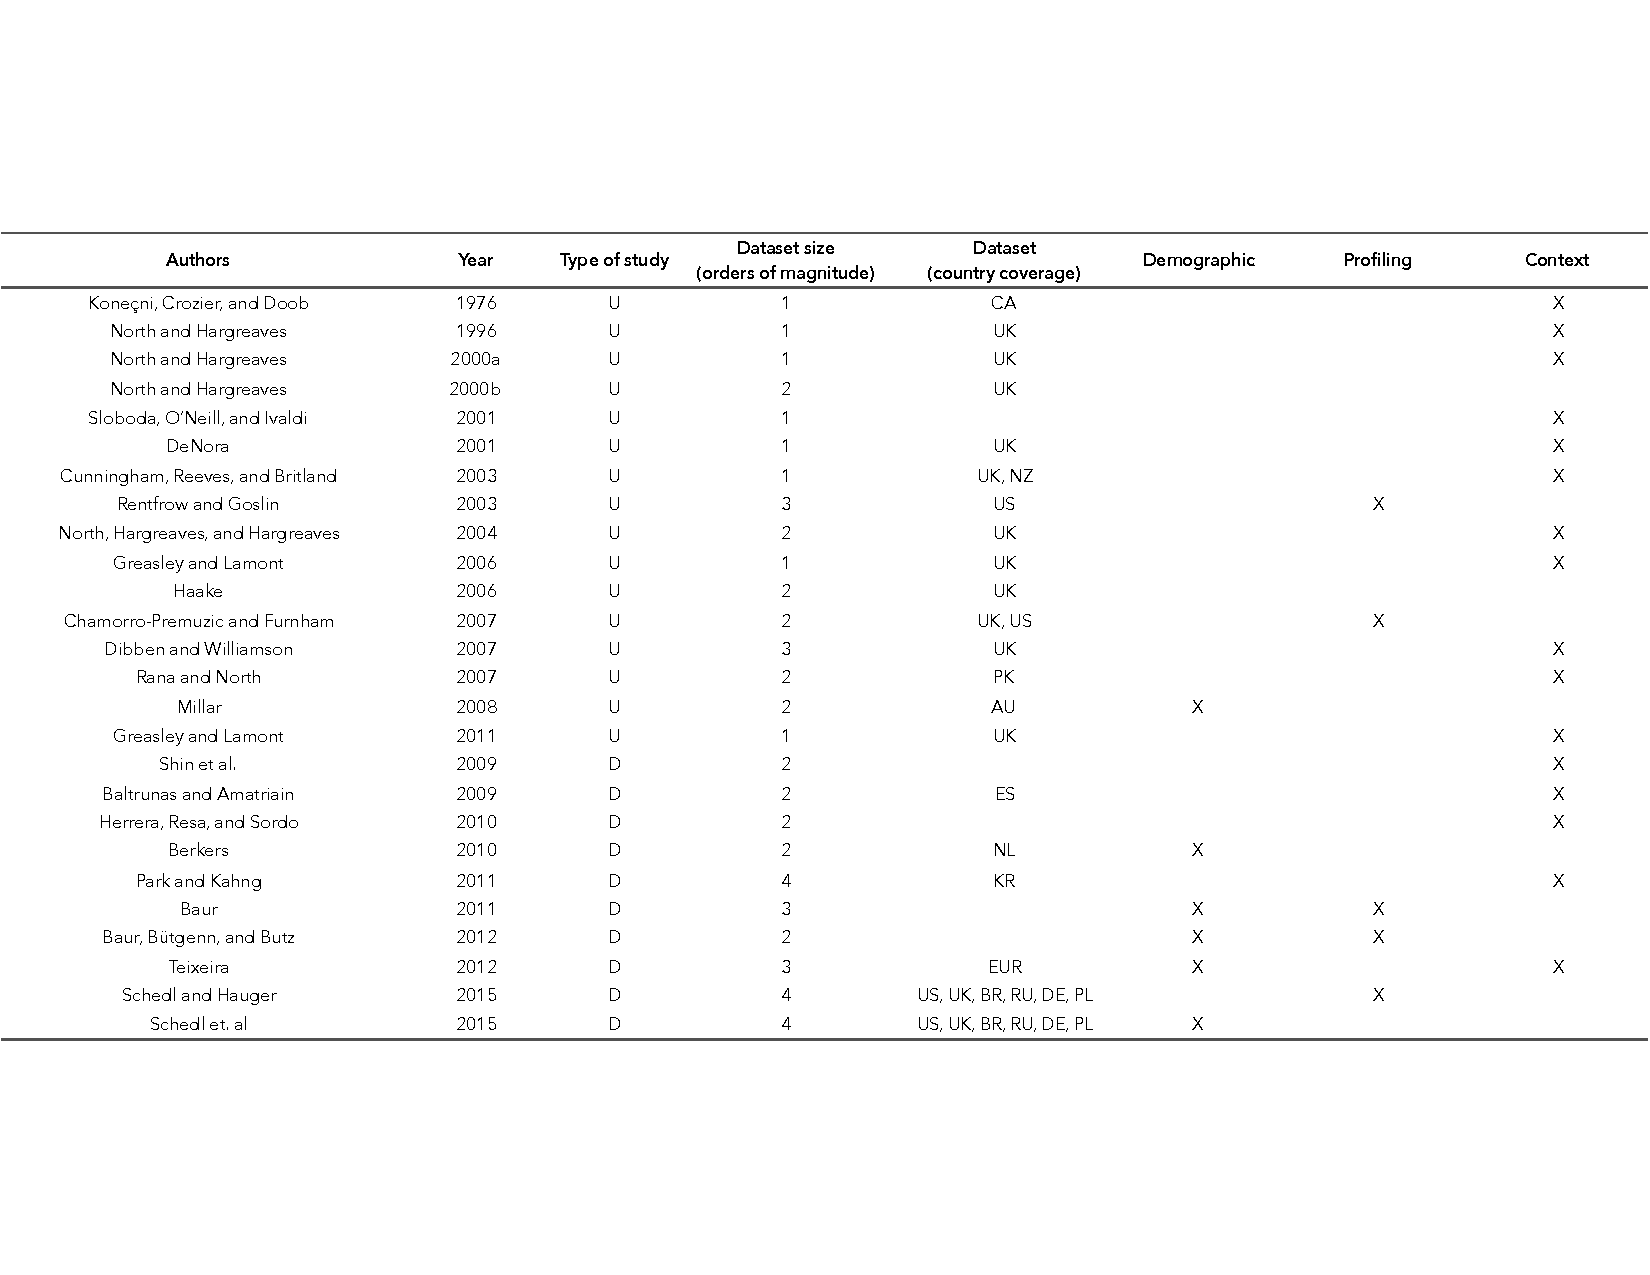
\includegraphics[width=1.0\linewidth]{figs/ch2/tabla_maestre.pdf}
%     \caption[Summary of previous studies about music preference and listening behaviour]{Summary of previous studies about music preference and listening behaviour in regard to the data of publication, the type of study (i.e., user-driven (U) or data-driven (D)), the size of the dataset used in orders of magnitude (i.e., ``1'' means 10--99, ``2'' means 100–-999, ``3'' means 1000–-9999, etc.), the geographical location of the people surveyed, and the use, or not, of user-centric features.}\label{tab:maestre}
% \end{sidewaystable}
% }


{\captionsetup[table]{belowskip=3cm, aboveskip=0cm, skip=-2cm}
\begin{sidewaystable}
    \centering
  \caption[Summary of previous studies about music preference and listening behaviour]{Summary of previous studies about music preference and listening behaviour in regard to the data of publication, the type of study (i.e., user-driven (U) or data-driven (D)), the size of the dataset used in orders of magnitude (i.e., ``1'' means 10--99, ``2'' means 100–-999, ``3'' means 1000–-9999, etc.), the geographical location of the people surveyed, and the use, or not, of user-centric features.}\label{tab:maestre}
  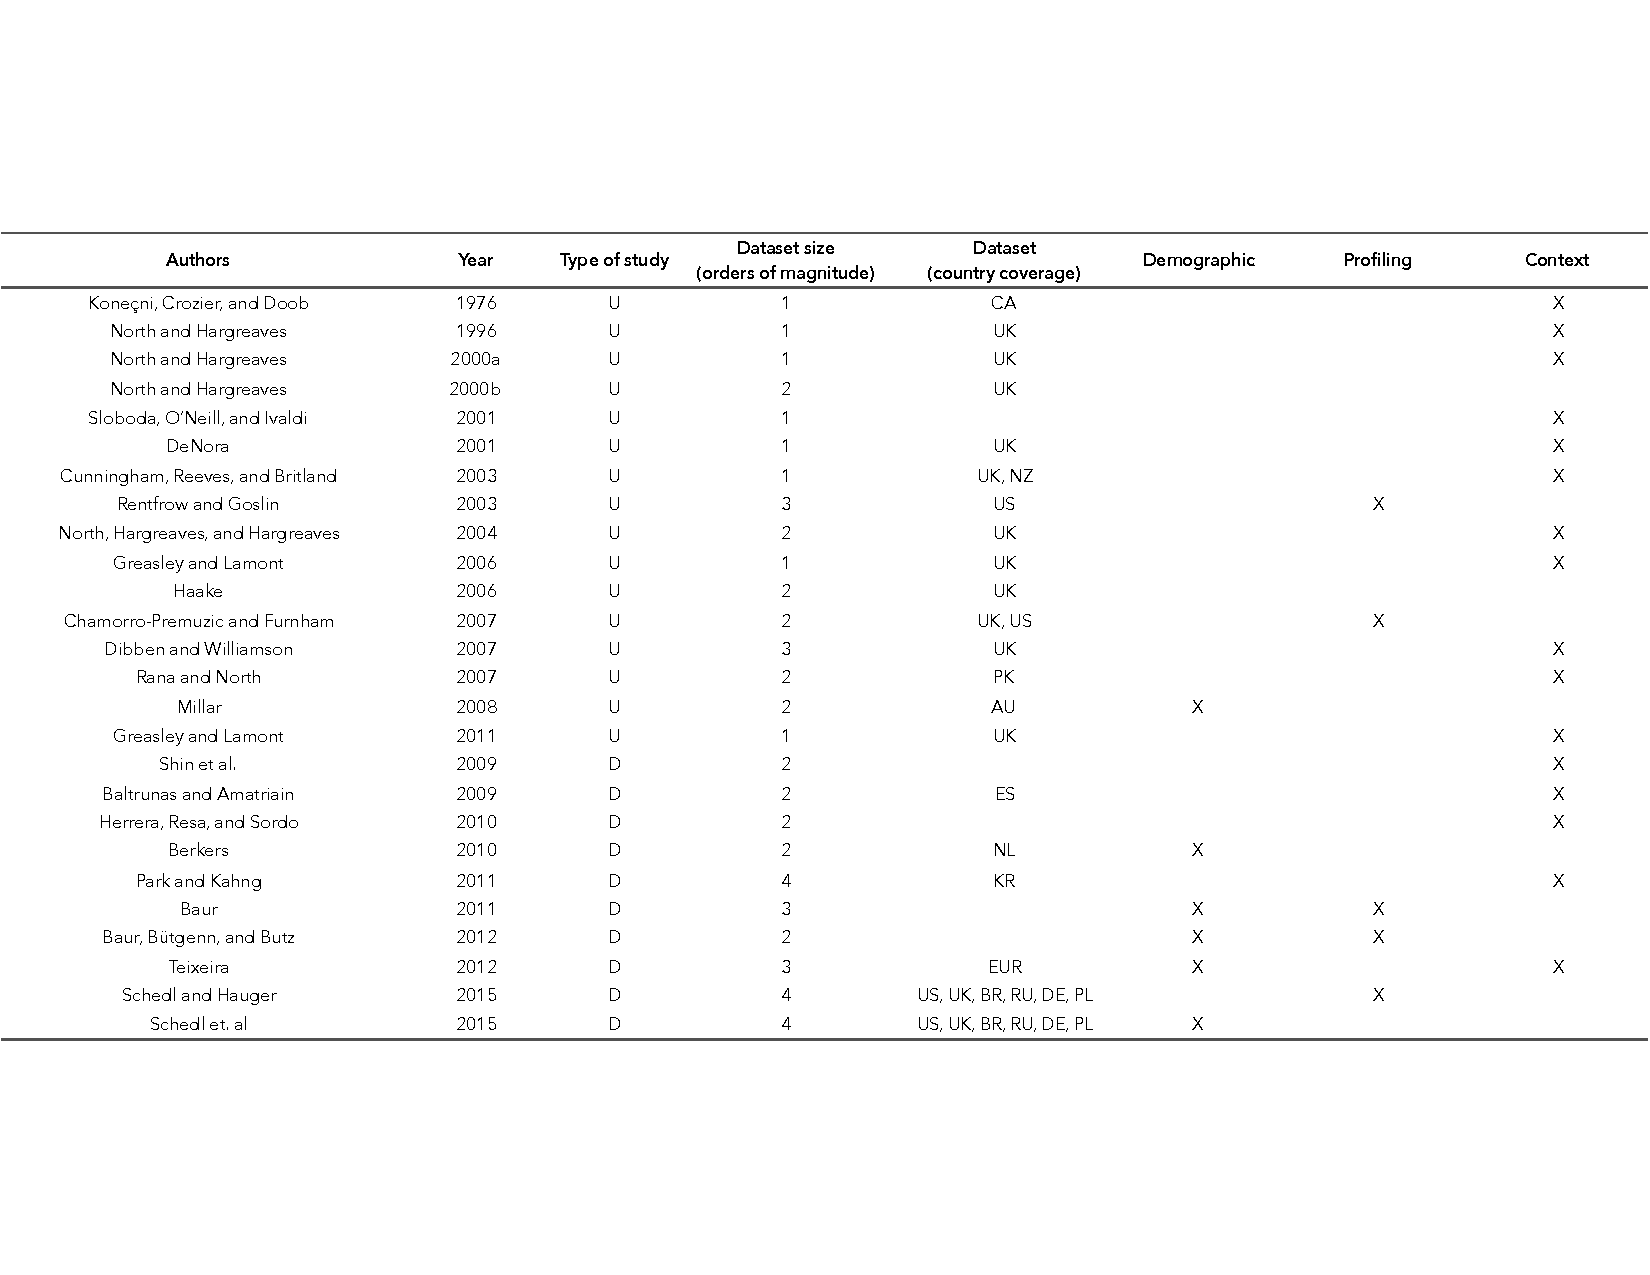
\includegraphics[width=1.0\linewidth]{figs/ch2/tabla_maestre.pdf}
  
\end{sidewaystable}
}


On the one hand, the table shows that a large number of user-driven research were carried out during the last decade. The data size of these studies was relatively small, in general. Mostly all research was carried out in the UK, with a few exceptions (e.g., \textcite{rana07role} evaluated previous research findings on anglophone populations, on listeners from Pakistan). The table does not show, however, that most of these studies were conducted in similar populations of listeners, usually undergraduate students in their late adolescence or early adulthood. 
In terms of user-centric characteristics (i.e., demographic, profiling, and contextual features), many user-driven studies correlated people's music preferences and their listening context, but their limited demographic coverage makes it difficult to extrapolate their results to a larger population. Also, just a few of these studies tried to correlate listeners' personality traits and music preference.




On the other hand, Table \ref{tab:maestre} also shows data-driven studies on people's use of music and music preference. Since data-driven approaches use a different method of data collection, we can see that the magnitude of datasets is larger, in general. Also, the more recent data-driven studies have expanded their geographic reach by collecting and analysing data of listeners from more countries, for example \textcite{schedl15tailoring} and \textcite{schedl15influence}. Also, it can be seen that data-driven studies have started to shift the research towards studying the correlations of people's demographic and profiling characteristics in regard to their music preference, for example in the studies by \textcite{baur11thesis} and \textcite{baur12listening}.

Finally, it is interesting to observe that none of the previous research used listeners' demographic, profiling, and contextual features all at the same time to study music preference. 
Since studying all these features at the same time can be difficult due to the expected large amount of interactions between them, we think that the best possible way of carrying out this  research is by using a very large dataset of music listening interactions. Consequently, this is the precise, specific spot where we want to establish our research: we aim to collect a large amount of music listening histories from a wide-reaching group of listeners, gathering or inferring their demographic, profiling, and contextual features, in order to evaluate if we can use these signals in the task of music recommendation.




% What are the main findings in people use of music in everyday life that could be applied to designing recommendation engines, particularly how they could be tuned to individuals taking all of these factors into account

\subsection{Application of listening factors into music recommendation systems} \label{sub:application_into_rec_sys}
We hypothesised that some of the previous findings on people's characteristics and music preference may be incorporated in the design of recommendation engines in order to help these systems to generate recommendations tailored to the specific features, habits, and contexts of listeners. 

First, as has been reviewed, listeners with different personalities use music in different ways, and so in designing and implementing novel recommendation engines, it seems reasonable to profile and typify the listeners according to their music listening behaviour, and fine-tune the recommendations to fulfil the specific needs and uses of each person.

Second, as music is usually chosen for accompanying a specific activity, it would be sensible to know what activity a listener is doing, is planning to do, or what are the specific moments in which those activities are frequently done. Thus, recommendations provided by systems might be used to distract listeners from their boring tasks, or for energizing and focusing people on their tasks, or for adjusting the meaning of specific activities or listening context by adding the significance of music. 

Third, as it seems that listeners change their listening behaviour and the music they listen to while in the company with other people, music recommendation systems should learn from these patterns in order to suggest music items that go along with these contexts. For example, a simple approach may consider asking listeners if they are using headphones. If so, a recommendation system may provide more serendipitous recommendations (i.e., recommendations that are surprisingly interesting that the user was not expecting) since listeners seem to be more adventurous while they are on their own.

Fourth, serendipity and coverage of music recommendation systems should be dependent upon the age of users. In other words, as previous studies found that older listeners are more inclined to  diverse music than youth, a recommendation engine should provide more serendipitous recommendations for this group. Music recommendations for teenagers, on the other hand, should stick to what they like.

Fifth, music suggestions provided to listeners by music recommender systems should consider their past listening behaviour. As suggested by previous studies, people have specific temporal listening patterns that may be exploited to generate better, more sensible recommendations.  


In the previous section we found that there is a lack of large-scale studies about people's use of music in everyday life using their demographic, profiling, and contextual features at the same time (see Table ~\ref{tab:maestre}). We also made clear that that is precise place where we want to establish our research: to perform a data-centric study of music listening behaviour and preference considering a large number of people and a set user-centric features.
In Section \ref{sec:3-big-music-data} we will describe the characteristics and technology needed to collect and analyse large amounts of data and in Section \ref{sub:music-data-sources} we will present a review of sources of music data. We will finalise this chapter in Section \ref{section:music_metadatabases} by presenting a comprehensive summary of all already available big music listening databases.








% \resetdatestamp
\section{Big Music Data}\label{sec:3-big-music-data}
% \setcounter{footnote}{0}
\graphicspath{{./figs/ch3/} }
The turn of the millennium also marked a turning point for the music industry. Recorded music sales declined abruptly due to the rise of peer-to-peer networks and online piracy. However, the number of yearly released albums continued growing steadily \autocite{frankel14evolution}. 
In this new music economy, the digital music consumption landscape has kept changing and growing in previously unseen manners. 
Perceptual-based audio compression algorithms and pervasive mobile Internet access allow listeners ubiquitous music listening. 
Listeners are currently witnessing the birth of new channels for listening to music, and experiencing it in new ways. People adapt their listening behaviour to these new mediums but they also influence them. For example, people are no longer interested in owning physical copies of recorded music or music files, they seem to be more than happy with just accessing services that provide the ability to listen to the music they want, whenever and wherever they like \autocite{wikstrom13music}.

% - connectivity vs control
% - service vs product
% - amateur vs professional

% This regular increase in the number of  albums and songs indicates that the volume of available recorded music information is ever-growing. 

Music streaming services nowadays centralise the access to a large part of the global music catalogue. These systems allow people to find and discover music by means of searching for the names of songs, albums, or artists; by browsing for categorical descriptors such as genre or mood; or by automatically generating recommendations or playlists that people may listen to and, perhaps, like. 
The recommendations generated by these systems are usually adaptive to what listeners have enjoyed, and so music services as well as listeners are learning about how to interact with each other.
Since all listening interactions can get stored, large amounts of music listening-related data are readily available for music listening behavioural analysis. 

% Economic models of these music services are based mainly on \emph{paid subscriptions}, that is listeners pay a fee for accessing a recorded-music database; or \emph{ad-based access}, by which listeners become the target of advertisement, usually tailored to their online listening behaviour. 

% Large amounts of data, hard to navigate


In the next subsections we will describe the main characteristics of big data, summarising the main evolving technologies associated with the processing and analysis of large amounts of information, and we will provide a comprehensive list of publicly-available databases of music listening information.


\subsection{Big data characteristics}\label{sec:3-big-data-characteristics}
Big data is a trending concept about which many lines have been written in the media and the music industry, as well as in academia. Its conceptual meaning, however, has been loosely defined, and largely depends upon the field that defines it. 
On the one hand, computer scientists are mainly interested in the array of technologies and algorithms to gather, store, and analyse large amounts of data, and so they tend to focus their work in these areas. On the other hand, humanists focus their research on the insights and social implications that can be extracted from social data by analysing people's digital traces \autocite{boyd12critical}. 
These simultaneous approaches are both essential in the discussion about big data because they provide different angles and points of view about this moving-target concept.
As a result, many questions regarding big data can be raised and attempted to be answered:
What technologies are and will be needed for dealing with ever-expanding data repositories? 
What kind of statistical approaches and machine learning algorithms will be needed to process and perform fast computational analyses on large datasets?
What kind of insights can be obtained from observing the online behaviour of people? 
Do these insights reflect people's actions and are hence generalizable to real-life?





\textcite{laney013d} postulated three properties that would characterise data management for the new millennium, and for which new technical approach\-es, formalisms, and technologies ought to be developed: \emph{volume}, \emph{velocity}, and \emph{variety}. Since then, these  defining features are known as the ``3 Vs,'' and are commonplace across literature on big data.

The volume axis refers to the idea of collecting, dealing, and processing ever-growing volumes of data. The size of big data repositories currently ranges from several terabytes to petabytes of data but, as the pace of growth of data is nowadays exponential \autocite{hilbert11world}, the amount of data that will be processed and analysed in the near future may  be as large as a few orders of magnitude bigger.

Velocity implies the ability of dealing with data that has to be collected, updated, processed, and analysed in real time, or near real time. Insights from the data, and decisions coming from these insights, may be needed on a daily basis, and so it is relevant to deal with the data rapidly.

Variety is a characteristic of big data that refers to having to deal not only with structured data---the type of data defined in database tables---but with semi-structured as well as non-structured data, such as social, mobile, video, audio data, or the combination of all of those. 
This characteristic makes big data management problematic, since all data fields can not be defined in advance, and the data structure and management should be able to deal with the many forms by which the data can be manifested.

Value has been lately mentioned as the fourth V.  It refers to the potential insights that can be extracted from the data, thus transforming them into value. This value can then be used by organisations to inform their decision making \autocite{manyika11big}. 

There is a general agreement in that the aforementioned properties describe inherent characteristics of big data, but there is still no formal definition for it. 
\textcite{demauro14big} studied the most recurrent keywords related to big data within abstracts of industry articles and scholarly articles from different disciplines, and found that  four different topics typically interact: information, technology, methods, and impact. 


% It has been commonly accepted, however, that big data deals with collecting large amounts of data into datasets, extracting information and getting insights from these datasets, the advances in technology needed to process and analyse massive repositories of data, but also with cultural shifts in business as well as society. 

% INFORMATION]

At the present time, vast amounts of data of various nature are constantly collected and processed.
Researchers from academia, private companies, and governmental organisations then use statistical methods and machine learning techniques in order to obtain insights from the data, thus converting raw data into information. 
For example, environmental data is collected by governmental agencies to predict future weather. 
Social data is collected by social media companies to tailor advertisement to users of their systems. 
Data about customer browsing or buying behaviour is used by online retailers to improve the sales of goods. 
Music listening or movie watching behavioural data is analysed by media streaming services to improve the satisfaction of users about their systems, to customise their exposure to advertisement \autocite{echonest13how} and, ultimately, to increase the retention of users in the services \autocite{gomez15netflix}.
% Also, large-scale digitization and datafication of books, for example, allow people today to look for terms through millions of books, and to researchers to search for patterns in the text of those books. 
% Nowadays, much data is also being generated by the many sensor-enabled, connected devices that people use, such as mobile computers or phones, providing real-time data about our actions and patterns in everyday lives. 




% TECHNOLOGY
\subsection{Technology}\label{section:technologies}
% http://transforming-musicology.org/resources/documents/methods-for-analysing-large-scale-resources-and-big-music-data.pdf
Technology plays an essential role in collecting, processing, and extracting insights from big data. Since the velocity of growth and the volume of data is larger every day, single workstations are no longer capable of processing massive datasets in a reasonable amount of time. This is a problem if real-time decision making is needed.

\textcite{moore65cramming} foresaw that the increase of the density of components in integrated circuits would double every two years, thus doubling the computing speed and the overall processing power and performance of computer systems. Although true for decades, Moore's law is nowadays no longer valid, since physical limits have been reached in terms of scaling the density and performance of CPU design \autocite{sheu15ep1}.

In response to the plateau in the clock speed of CPUs, a number of approaches based on the idea of aggregating individual computer power have been developed in order to obtain the high performance needed to process big data repositories.
High Performance Computing (HPC) systems are clusters of single computers known as nodes. Each node has multiple processors and each processor has multiple cores. 
Fast and reliable network connections between nodes are needed to allow rapid intercommunication between nodes.
On top of these systems, a number of technologies have been developed in order to deal with parallel and distributed processing of large amounts of data. The most commonly used technologies are the Message Passing Interface (MPI), Hadoop, and Spark.

% https://github.com/ljdursi/mpi-tutorial/blob/master/presentation/presentation.md
MPI (1991) is a standardised communication protocol for passing mes\-sages---the MPI basic level of abstraction---to parallel processes on HPC systems. MPI is structured as a library with an application programming interface (API). The MPI API has a series of operations to explicitly send and receive messages from specific or all nodes. 
MPI systems use distributed memory, meaning that MPI parallel threads do not share memory. Therefore, if a thread needs data from another thread, the data transfer between them has to be explicitly coded, and the data is transferred through the network. 
MPI is not fault tolerant, meaning the user has to explicitly take care of handling possible errors in any of the nodes.

% OpenMP is another system for message passing. In this case, however, all nodes in the cluster have a \emph{shared memory} space, and so the communication between parallel threads happen in memory. This implies that all execution threads need to be in one physical machine.


A more recent technology for parallel computing is Apache Hadoop (2007). It is an open source implementation of Google's MapReduce \autocite{dean08mapreduce} distributed computational model, running on the Hadoop Distributed File System (HDFS) \autocite{shvackho10hadoop}. 
Unlike MPI, Hadoop provides automated means for scaling processes across nodes and a tolerance system for dealing with failures in any of the parallel processes. 
Hadoop is a technology of higher level than MPI, meaning that a user can specify the computational process needed in terms of custom-written map and reduce functions---to parallelise processes and aggregate their results respectively---and the system will scale the processes to the cluster size. 
In other words, Hadoop itself will handle the parallelism, scheduling the computations across the cluster and balancing the processing load across nodes without human intervention. 
Fault tolerance, the ability of a system to deal with failures, is implemented in Hadoop by means of automatically splitting data files into blocks, replicating them by a user-defined factor (typically a factor of three), and finally shuffling and distributing them across nodes. 
This fault tolerance procedure ensures that if a process in a node fails, the master node will trigger the processing of the replicated version of the same block in another node. 
Because of its fault tolerant capabilities and its scalability, Hadoop was a step forward for the processing of large datasets in comparison with MPI. 
However, it is not efficient for routines that reuse a portion of data across multiple operations, such as iterative jobs or interactive analytics applications.
The former case is usually used in machine learning algorithms, where a function is applied repeatedly to the same dataset in order to iteratively optimise a parameter. 
In cases like this, Hadoop reloads data from disk for each iteration. As a result, the performance of the system is diminished.
In interactive analytics tasks, several queries are performed on the same dataset interactively by a user. In this case, Hadoop treats every query as a new MapReduce job, reading all data from disk every time, which also slows the performance of the system.
% https://github.com/ljdursi/hadoop-for-hpcers-tutorial/blob/master/presentation/presentation.md

Apache Spark \autocite{zaharia10spark} is a cluster-based computing framework developed to overcome the drawbacks of Hadoop for applications that reuse a working set of data. 
It has scalability and fault tolerance characteristics that are similar to Hadoop's, but it is based on a core abstraction named Resilient Distributed Dataset (RDD). 
An RDD is a read-only collection of objects which can be partitioned and distributed through nodes of a cluster. If by any reason a partition is lost, it can be reconstructed from the rest of the dataset. RDDs can be cached in memory across machines in order to reuse them for multiple distributed parallel operations, therefore speeding up calculations. It is also possible to use an interpreter to work interactively  with the RDDs and perform parallel operations on a cluster.
Although Spark runs on HDFS, it can also run on other file systems, allowing Spark to be deployed in pre-existing HPC frameworks, which is not possible with Hadoop. 




In order to obtain useful insights from big datasets, the data have to be processed accordingly in order to be able to cope with their unique characteristics of volume, velocity, and variety. 
% Different analytical methods  
% Traditional techniques derived from statistical methods are \emph{regression}, \emph{correlation}, and \emph{factor analysis}. These techniques allow to reveal dependence relationships between a variable and other variables, and to determine the law of correlations that describe the many variables of a phenomena. 
However, traditional analytical methods and techniques for recognising patterns from datasets have to be adapted in order to deal with the intrinsic characteristics of big data. 
As seen previously, processing large volumes of data, one of the characteristics of big data, has been mainly addressed by the development of computational tools that allow for efficient data parallelisation. 
Modern data mining algorithms take advantage of this parallel processing by means of splitting large datasets into several threads, the results of which are later combined into a single machine for the analysis.

The technologies used in big data are agnostic to the specific type of information that is being processed and analysed. 
Therefore, these techniques can be applied to complex manifestations with many sources of information, such as music.
In the next section, we will provide a review of the different types of music information, as well as different repositories and databases that offer this information. Data in these sources represent different aspects of music and music listening behaviour, and so we will examine them in order to decide which ones can provide data for studying how to improve a music recommendation model by means of user-centric features. 



% Data mining aim to extract uncover useful information and insights from the data by means of applying different data mining techniques.
% The next section provides a review of data mining techniques to process large amounts of data. 





% \section{Techniques}\label{section:techniques}

% One of the goals of analysing large datasets is to discover unknown trends and facts within the data. These trends can then be used to get insights that may inform decision-making. 
% \emph{Knowledge extraction} uses the insights learned from analysing data to explain the data characteristics and behaviour.

% In classification, class labels are assigned to data with previously unknown labels. Prediction tasks, on the other hand, try to estimate the outcome of a given set of input data or signals. 




% Classical tasks for music data mining are: %http://users.cis.fiu.edu/~lli003/Music/music.html

% \begin{description}
% \item [Association mining]
% \item [Classification] Genre classification, rhythm classification, artist classification, mood detection and classification, instrument classification and recognition, singer identification
% \item [Clustering]
% \item [Sequence mining]
% \item [Similarity search]
% \item [Music summarisation]
% \item [Music visualisation]
% \item [Music indexing]
% \end{description}

% % Write about MIREX as the milieu where state-of-the-art techniques for music data mining are tested and benchmarked

% classical tools and algorithms for data analysis are adapted in order to take advantage of parallel processing. 

% \emph{Big data analytics} is the application of advanced analytical tools, such as data mining, statistics, predictive analysis, or machine learning, to very big datasets.

% These techniques include supervised approaches, such as classification and regression, and unsupervised approaches, such as dimensionality reduction through clustering or topic modelling. 

% Models are called \emph{predictive} if they are used to predict class labels on data with unknown labels, or \emph{descriptive} if they are used to obtain knowledge from the data. \emph{Knowledge extraction} is the action of using the rules from learned models to explain the data characteristics and behaviour. % \autocite{mckay10automatic}

% More complex models can be used to explain the data variability as the size of datasets increase, without risking to over-fit the data.






\section{Music data sources}\label{sub:music-data-sources}
There are several sources of music-related information currently available. Some of them are commercial services that provide paid access to their data, and others are crowdsource-based services that allow free access to data protected with Creative Commons licenses or is in the public domain.
These repositories provide information that represents different aspects of music, such as music metadata, acoustic features, lyrics, music reviews, social tags, non-audio representations, and music listening histories.
We will now describe the different types of musical data and related metadatabases.

\begin{description}
\item [Music metadata] Metadata is structured information that identifies, describes, locates, relates, and expresses different layers of data about an information resource \autocite{dcmi12dublin}. The \textcite{niso04understanding} declared three basic types of metadata: descriptive, for purposes such as identification and discovery;  structural, for expressing relations among resources; and administrative, for managing resources. 
In the music context, descriptive metadata commonly provides information about recordings, such as the song title and length, the artist name, and the release name. This information is usually stored in an MP3 ID3 tag or in chunks of the audio file especially designed to represent this information. However, music metadata can also provide structural information about attributes not necessarily linked to an actual recorded piece of music, such as a song's track number within an album or a playlist, linking song names to video clips, or artists to their biographies, for example. 
As a results, music metadata adds value to the musical object because it helps to mediate and enhance the experience of listeners with music and artists, allowing them to browse, explore, sort, collect, use, and finally enjoy music. 

A few music metadatabases provide commercial metadata of musical artists, releases, and songs to digital music services. Rovi Music\footnote{Rovi acquire the company Tivo, and now it can be accessed via Tivo's Web site at \url{https://business.tivo.com/products/music-metadata.html}} and Gracenote\footnote{The Gracenote Rhythm metadata service website is available at \url{http://www.gracenote.com/music}} are among the databases with the longest history. Allmusic\footnote{The online music guide service AllMusic is available at \url{http://www.allmusic.com}} uses Rovi data, but it adds reviews and creates free personalised recommendations to registered users. 
Quantone\footnote{Quantone provides semantic music metadata for media companies. Its website is available at \url{http://quantonemusic.com/}}offers paid programmatic access to extended metadata and additional information on artists, albums, and tracks. 
Data licenses for all these databases are restricted. 

On the other hand, there are a few user-built, open-data, music metadataba\-ses that provide less restricted access to music metadata. Most data in these databa\-ses is in the public domain, which means that there are no restrictions in its use.
FreeDB\footnote{The FreeDB database of compact disk track listings is available at \url{http://www.freedb.org/}} is a database of CD track-listings from user-contributed data, originally based on the Compact Disc Database (CDDB).
MusicMoz\footnote{The MusicMoz directoryof community-curated information about music is available at \url{http://www.musicmoz.org/}} is a user-contributed database that stores music-related factual data and Internet links.
Discogs\footnote{The Discogs database and marketplace are available at \url{http://www.discogs.com/}} is a large, user-populat\-ed database of discographies and music releases from physical sources. It provides high-quality data that is ensured by a strict input form mechanism and a large community of users.
MusicBrainz\footnote{The MusicBrainz music database is available at \url{http://www.musicbrainz.org/}} is a large, community-based, user-con\-tributed metadatabase that stores descriptive, structural, and administrative metadata for any kind of music release. Its high-quality database is constantly developed and enriched by an open community of users that negotiate periodically and consistently, with strict standards and routines, about the orientations, developments, style guidelines, and mostly everything on MusicBrainz \autocite{hemerly11making}. 
Music metadata can be obtained from these music metadatabases by means of online browsing or by accessing them programmatically through their APIs.

\item [Acoustic features] Music acoustic features are numerical representations of the audio signal that characterise some aspects of the signal.
Features are computed from the time or frequency representations of the audio signals, and describe their spectral, rhythmic, tonal, or other low-level or high-level characteristics. 
Comprehensive reviews and thorough description of audio features can be found in \textcite{tzanetakis02manipulation} and \textcite{mckay10automatic}.
Algorithms for calculating these feature-numbers have been developed by many music research groups throughout the years, many of which have been part of the Music Information Retrieval Evaluation eXchange (MIREX),\footnote{The MIREX competition website is available at \url{http://www.music-ir.org/mirex/wiki/MIREX_HOME}} which is an annual evaluation contest with the goal of comparing state-of-the-art algorithms relevant to music information retrieval tasks using same datasets and evaluation procedures \autocite{downie08music}. 

Acoustic features can be computed by using open-source software frameworks, stand-alone applications, or libraries such as Marsyas\footnote{The Marsyas software framework for audio processing is available at \url{http://marsyas.info/}} by \textcite{tzanetakis00marsyas}, the CLAM music annotator by \textcite{amatriain05clam}, jAudio\footnote{The jAudio program for audio feature extraction is available at \url{http://jaudio.sourceforge.net/}} by \textcite{mckay10automatic}, Aubio by \textcite{brossier06automatic}, the MIRToolbox by \textcite{lartillot08matlab}, and the VAMP plugins.\footnote{The VAMP audio analysis plugin system is available at \url{http://vamp-plugins.org/download.html}} 
The latter ones are used within host sound editor applications such as Sonic Visualiser or Audacity. 
The Spotify music streaming service also now encapsulated The Echo Nest API and provides a publicly accessible interface\footnote{Some components of The Echo Nest API are now available as part of the Spotify Web API available at \url{https://developer.spotify.com/web-api/get-audio-features/}} that allows the extraction of a collection of proprietary audio features based on the work by \textcite{jehan05creating}.


A few databases also provide open and public access to sets of already-computed acoustic features from a large dataset of songs. 
The Million Song Dataset (MSD) \autocite{bertin11million} provides metadata and a set of acoustic features for about one million songs, computed using the already mentioned custom features developed by \citeauthor{jehan05creating}. His approach relies on segmenting the audio signal where perceptual onsets occur instead of segmenting the signal using a fixed-length window. Then, a set of acoustic features is computed for each segment between onsets. 



Whereas the MSD corpus was a centralised database of a fixed size, AcousticBrainz\footnote{The AcousticBrainz API, datasets, and data are available at \url{https://acousticbrainz.org/}} is a crowd-sourced distributed initiative that relies on contributions from a large number of users performing feature analysis in their own music collections\autocite{porter15acousticbrainz}. 
It provides a small application that can be downloaded for free and performs the metadata validation, features analysis, and feature delivery to the database. 
AcousticBrainz' feature analysis computation is accomplished by the Essentia\footnote{The Essentia library for audio analysis and audio-based music information retrieval is available at \url{http://essentia.upf.edu/}} audio analysis library \autocite{bogdanov13essentia}, which computes a comprehensive set of features with fixed-window size.

Since AcousticBrainz was conceived as a crowd source project, it is ever-expanding, and less biased than the MSD dataset of acoustic features. However, it is perhaps more prone to errors, due to possible discrepancies in people's music collections due to duplicated and different versions of music files (i.e., AcousticBrainz stores every acoustic feature analysis submitted by its users, and so it is not uncommon to find in its database songs that have a set of feature values totally different, for the same songs).


\item [Lyrics] Songs usually comprise a set of words complementing and reinforcing the music, and so the act of listening to a song involves being exposed to the text as well as the music, as a single message.   Therefore, song lyrics are an important component in the appreciation of musical pieces that has received little attention in music research in comparison to audio analysis, for example.
Moreover, lyrics are contained within the audio signal but extracting  text directly from music recordings is still a hard task. Hence, many websites offer access to human transcriptions of lyrics. Some of these sites allow public access to user-contributed lyrics and others are paid services that permit programmatic querying for industry-approved lyrics. 
Examples of the former are 
Musixmatch\footnote{The Musixmatch website and database are available at \url{https://www.musixmatch.com/}} and 
AZLyrics.\footnote{AZLyrics is available at \url{http://www.azlyrics.com/}} 
Lyricfind,\footnote{The lyrics licensing company LyricFinding is available at \url{http://www.lyricfind.com/}} 
ChartLyrics,\footnote{ChartLyrics is a community-driven database of lyrics. Its website and API are available at \url{http://www.chartlyrics.com/}} and 
MusicStory\footnote{MusicStory is a metadata provider that also supplies lyrics via an API available at \url{http://developers.music-story.com/developers/lyric}} are examples of the latter.

\item [Music reviews] Publicly available reviews of music items such as albums, songs, videoclips, concerts, or artists carry information about how people perceive these music items. Since music enjoyment has a social component, and people's perception on music items seems to be mediated by the context of listening, music reviews can be a rich source of cultural information about how listeners assimilate and perceive musical items. 
The Internet is the place where the largest amount of these music items are currently released and it is also the place where most people write  and share their impressions about music. 
Moreover, music reviews do not only deliver people's opinions about music, but also a large amount of information concerning the background and context of the music items.
There are many websites that provide music reviews but just a few of them offer programmatic ways of accessing their information. Among these websites, the largest ones are
All Music Guide,
RollingStone,\footnote{The American magazine focused in popular culture and music RollingStone is available at \url{http://www.rollingstone.com}} Pitchfork,
\footnote{The American online magazine Pitchfork is available at \url{http://www.pitchfork.com}} 
Metacritic,\footnote{Metacritic aggregates reviews of music and media in general. Its website and database are available at \url{http://www.metacritic.com/music}} 
Rateyourmusic,\footnote{The online collaborative metadatabase of music and media is available at \url{http://rateyourmusic.com/}} and 
Stereogum.\footnote{The online publication Stereogum is available through its website at \url{http://www.stereogum.com}}

% Allmusicguide belongs to Rovi (at least from their API key access), API seems to be inactive

\item [Music social tags] Social tags are free keywords assigned by listeners to specific music items. These labels express the independent thoughts of listeners on music, and so they convey a large amount of human-generated contextual knowledge in the form of descriptive text that  goes beyond standard music metadata. 
As tag fields do not have restricted categories, they capture the free appreciation of people on music. 
As a result, common tags of music items can express music genre, emotion, decade, instrumentation, or any word capturing some aspect of people's perception of music. 
The aggregated collection of tags is known as a folksonomy.  
A few music services allow users to tag music items within their own ecosystem, or through other music applications that submit and retrieve the tags from their databases. Currently, the largest of these services offering APIs to digitally retrieve the labels are Last.fm and MusicBrainz, though the former has a much larger amount of music items tagged. 
However, \textcite{lamere08social} pointed out that one drawback of social tagging is that usually only popular items get tagged.
Therefore, in order to avoid this popularity problem, the collection of music-related metadata using free text labels has also been done using  music ``games with a purpose.''
\textcite{mandel08web} developed MajorMiner, a game that collected music tags by means of single-player free tagging of 30-second music clips. Agreement with previous tags provided points, and tag trend-setters received extra bonus points.  
In The Listen Game, \textcite{turnbull07game} asked users to choose the best and worst from a fixed set of music tags for 30-seconds music clips. 
\textcite{kim08moodswings} required people to express the mood carried by musical pieces in a two-dimensional grid of arousal and valence of their game Moodswings. 
Finally, \textcite{law09input} developed an online game to collect tags for music and sound clips named TagATune that was collaborative in nature. Two participants were asked to tag a track but they did not know if it was the same. By the end of the tagging process, the users expressed if they were actually listening to the same tune or not. Participants received points if their guess was correct. 
The approach by \citeauthor{law09input} incremented people's retention in the game, receiving a larger number of tags and incrementing the number of verified tags.
Eventually, \textcite{law09evaluation} assembled a dataset with all data collected with the game and made it available as the MagnaTagATune Dataset.\footnote{The MagnaTagATune Dataset website provides access to the dataset, audio clips, audio features, and similarity data at \url{http://mirg.city.ac.uk/codeapps/the-magnatagatune-dataset}} This set was made public and was used for an audio tag classification task at MIREX 2008.



% \item [Symbolic music]
\item [Non-audio representations]
% Music can be represented by various means. The audio rendering of a piece of music is just one of the many instances that a music piece can have. 
A large number of websites provide music in many non-audio representations. These renditions can be visual representations of music scores, Musical Instrument Digital Interface (MIDI) files, or transcriptions of music encoded into symbolic music formats. 
These symbolic music representations encode music symbols within a file that attempts to preserve the relationships between the elements of the score.

Visual representations of music scores are provided as downloadable PDF files by websites such as the International Music Score Library Project\footnote{The Petrucci Music Library is available at \url{http://imslp.org}} or Music Scores.\footnote{\url{http://www.music-scores.com/}} Moreover, images of original scores are hosted by international virtual libraries and can be inspected using image viewing platforms. Examples of these libraries are the Digital Image Archive of Medieval Music\footnote{The Digital Image Archive of Medieval Music website is available at \url{http://www.diamm.ac.uk/}} and e-codices.\footnote{The e-codices website provides access to all the digitised manuscripts in their database by means of a virtual library available at \url{http://www.e-codices.unifr.ch/en}}  The Cantus Ultimus project\footnote{The Cantus Ultimus project is available at \url{http://cantus.simssa.ca/}} also delivers symbolic music information aligned to zones in the score image. 
The Musiclibs\footnote{The Musiclibs image search system is available at \url{https://musiclibs.net}} project is a document image search system that allows searching within collections of digitised music documents located in different institutions across the world using a single interface. Musiclibs works by aggregating International Image Interoperability Framework (IIIF) manifests\footnote{The IIIF documentation for manifests is available at \url{http://iiif.io/api/presentation/2.1/#manifest}} served by international libraries. By means of these manifests the images are served directly from the originating organisation's repositories. Musiclibs does not cache or display images directly.

Symbolic representations of music using the MIDI protocol encode, at the very least, the timing, pitch, length, and velocity of notes. The MIDI protocol has been the digital music instruments industry standard for the past 30 years and so it is widely used in the context of music production. 
Its standardised data, and the fact that provides a large amount of musical information in a small file size, has facilitated a large number of websites devoted to sharing music in MIDI format, enabled by a large community of people creating these files. 
However, since international copyright law restricts the ability to make copies of musical works for a fixed amount of time before going into the public domain, many MIDI files of recent creations are offered as paid files. Creations that are already in the public domain can be free or licensed, depending on if the MIDI rendition is protected by a performer's performance copyright.
Hit Trax,\footnote{The Hit Trax website with MIDI-based karaoke backing tracks is available at \url{http://www.hittraxmidi.com/}} Classical Archives,\footnote{The Classical Archives website of MIDI files is available at \url{http://www.classicalarchives.com/}} and MIDI World\footnote{The MIDI world website and data is available at \url{http://www.midiworld.com/}} are among the largest free and pay websites.


\item [Music listening histories] Music listening histories are records of music listening events. These records are typically expressed as a series of logs indicating at least the time and date of the listening event, the music items that were played back, and the identification of the user account associated with the media player application.
Earlier in this chapter, we detailed  a number of applications that collect local and global data of music listening logs (see Section \ref{sub:data-driven studies} in particular). However, only some of those applications offer their music listening data for public analysis and research. 
As one of the main focuses of this dissertation is to perform a large-scale data-driven study about music listening behaviour, in the next section we will provide an extensive review of music listening databases.
\end{description}













\section{Big music listening databases}\label{section:music_metadatabases}
\graphicspath{{./figs/ch4/} }
We are interested in evaluating the impact of using demographic and profiling features, as well as contextual information, on the performance of a music recommendation model. A few publicly available datasets for music listening research provide information relating a large number of people and music items. We will now review those datasets.

\begin{description}
\item [Yahoo! Music Dataset] 
Yahoo! released in 2011 a dataset of user ratings collected through its Music Radio service.\footnote{The Yahoo! Music dataset with user ratings of musical tracks, albums, artists and genres is available at \url{http://webscope.sandbox.yahoo.com/catalog.php?datatype=c}} In the KDD-Cup'11, Yahoo! challenged the music informatics research community to identify users' listening tastes by assigning the task of predicting users' rating on musical items in the test data of the dataset \autocite{dror11yahooa}.
The original version of the dataset had more than 262M ratings from 1M users, on 625K musical items including: tracks, albums, artists, and genres. These items were linked into a 4-level hierarchical structure. 
Each user in each dataset had at least 20 ratings on music items. 
In order to protect the privacy of users, their user names as well as musical items' identity were relabelled. Also, the dataset did not provide any demographic information about the listeners. Yahoo! released the dataset in a couple of versions with similar characteristics but with different sizes. 
In order to learn, apply, and generalise insights from the data, Yahoo! released each version of the dataset into splits of training, validation, and test subsets. 
While the validation and test subsets had four and six of each set of user ratings, the training subset had all the rest of ratings per user. 


The results of the Yahoo!-KDD competition reinforced some of the findings already posed by \textcite{koren09collaborative,koren09bellkor,toscher09bigchaos} in the domain of movie recommendation: the modelling of temporal changes in users' behaviour and items' popularity, and the blending of multiple techniques of collaborative filtering enable a large improvement in performance of a recommendation model.\footnote{These findings were part of the methods used by the winner team of the Netflix prize. Details about this competition will be given in Subsection \ref{sub:netflix}.}
% The Yahoo!-KDD competition reinforced many of the findings on the Netflix data, where solutions were created by blending multiple techniques, and modelling temporal changes in users' behaviour and items' popularity was essential for improving solution quality. 
Wisely, \textcite{dror11yahoo} concluded their account of the results of the competition with an open question about ``...whether small improvements in RMSE terms can have a significant impact on the quality perceived by real user.''




% 252800275/262810175 = 0.962
% 4003960/262810175 = 0.015
% 6005940/262810175 = 0.023


\item [Echo Nest Taste Profile subset] 
The Echo Nest introduced in 2011 the Taste Profile subset, a dataset of user playcounts tailored to user-centric music recommendation research \autocite{mcfee12million}.\footnote{The Echo Nest's Million Song Dataset Taste Profile subset is the official user dataset of the Million Song Dataset. It is available at\url{http://labrosa.ee.columbia.edu/millionsong/tasteprofile}}
The dataset consisted roughly on 48M music listening logs of undisclosed origin, gathered from  listening histories of 1.2M users on 380K songs, and formatted as triplets \texttt{<userID, songID, count>}. Unlike the Yahoo! Music Dataset, the Taste Profile dataset provided playcounts instead of ratings, and so it represents implicit instead of explicit preference. The song IDs in the subset were based on Echo Nest identifiers and so they matched complementary datasets in the MSD. This linkage allowed researchers to link artists' biographical information, song lyrics, audio content analysis, online artist popularity measures, album covers, artist tour dates, song and artist tags, artist and song similarity metrics, and 30-seconds audio snippets for most songs \autocite{bertin11million}. The dataset did not provide timestamps of the music logs or demographic information about the listeners.

The associated Million Song Dataset Challenge\footnote{The ``Million Song Dataset'' Challenge is available at \url{http://www.kaggle.com/c/msdchallenge}} was simultaneously released with the Taste Profile subset with the goal of predicting the songs that a user will listen to. Participants were encouraged to use all additional available data, and song content analysis data by means of shared music item identifiers with the MSD \autocite{bertin11million}. 
Recommendation algorithms were evaluated by recalling positively associated items for each user, in the form of evaluating the predicted ranking of songs \autocite{mcfee12million}. 
There is no official publication about the results and insights obtained from the Million Song Dataset Challenge, but the winner submission outperformed all other submissions by using an approach based on a single algorithm that computed similarities between users' playcounts, without using any of the other sources of data \autocite{aiolli12preliminary}.



\item [Last.fm Dataset-360K] \textcite{celma10music} introduced a dataset featuring artist playcounts for 360K unique users of the Last.fm music service.\footnote{The Last.fm Dataset - 360K users is available at \url{http://www.dtic.upf.edu/~ocelma/MusicRecommendationDataset/lastfm-360K.html}} 
The dataset contained MusicBrainz identifiers for artists and their playcount number per user. Each user was also characterised by the demographic features: gender, age, country, and registration date.

\item [Last.fm Dataset-1K] \textcite{celma10music} also introduced a dataset of full listening histories of almost 1K users.\footnote{The Last.fm Dataset with full listening histories from 1K users is available at \url{http://www.dtic.upf.edu/~ocelma/MusicRecommendationDataset/lastfm-1K.html}} These listening histories included user, timestamp, MusicBrainz identifiers for artists and songs, as well as names of artists and songs. Users were characterised by the self-declared demographic features gender, age, country, and registration date.

\item [HetRec2011-last.fm-2k] \textcite{cantador11workshop} presented a dataset\footnote{The dataset HetRec2011 is available at \url{http://files.grouplens.org/datasets/hetrec2011/}} with Last.fm data about listening counts for the 50 most listened artists of 2K users, accounting for a total of 18K artists. The dataset also included bi-directional friend relations and time-stamped artist's tags assignments per user. The dataset did not provide demographic information about users. 

\item [EMI 1 Million Interview Dataset] \textcite{emi12million} promised a dataset of 1M interviews about people's music appreciation, behaviour, and attitudes.\footnote{General information about the EMI 1 Million Interview Dataset is available at \url{http://musicdatascience.com/emi-million-interview-dataset/}} Available data in the set had ratings of users on EMI artists and tracks after a controlled listening test; a set of free words that people used to describe the artists and tracks, and demographic, personal; and music listening behavioural information about users. However, only partial information has been available so far, and no results or insights have been published.\footnote{A small subset of the EMI  EMI 1 Million Interview Dataset was released at the EMI Music Data Science Hackathon in 2012. The subset is available at \url{https://www.kaggle.com/c/MusicHackathon/data}}

\item [MusicMicro 11.11--09.12] \textcite{schedl13leveraging} introduced a dataset of listening logs extracted from Twitter \emph{tweets}, designed for studying spatial and temporal relations to music listening.\footnote{The MusicMicro corpus of music listening behaviour inferred from microblog data is available at \url{http://www.cp.jku.at/datasets/musicmicro/}} The dataset comprised 600K music-related logs, generated from 137K users on 20K unique artists. Tweets in the dataset originated from 21K different cities in 180 different countries.
The dataset consisted of tweets with any of the tags \texttt{\#nowplaying}, \texttt{\#np}, or \texttt{\#itunes}, that explicitly had precise location data. \citeauthor{schedl13leveraging} only provided tweets whose artist or song name could be linked to MusicBrainz and excluded all logs with the sub-string ``radio'' in order to suppress logs submitted by radio stations.
Therefore, each entry in the dataset provided time-stamped temporal and spatial data (i.e., longitude, latitude, country, and city), as well as custom-built user, artist, and track identifiers. The dataset did not provide links to other music metadatabases.


\item [Million Musical Tweets Dataset (MMTD)] \textcite{hauger13million} introduced a dataset of listening histories inferred from Twitter posts.\footnote{The MMTD corpus of music microblogging behaviour is available at \url{http://www.cp.jku.at/datasets/MMTD/}} The authors collected micro-blog posts using any of the keywords \texttt{\#nowplaying}, \texttt{\#np}, \texttt{\#thisismyjam}, \texttt{\#musicmonday}, or \texttt{\#itunes} during the lapse of 17 months.
The dataset comprised a total of 1M geolocalised logs from 215K different users. Each entry in the dataset provided custom-made user identifiers as well as temporal (i.e., date, time, time zone), spatial (i.e., longitude, latitude, continent, country, and city), and contextual information (i.e., country's demographic information) per log. Most artists were linked to MusicBrainz and a proportion of tracks were resolved to 7digital\footnote{The 7Digital music listening platform and API are available at \url{https://www.7digital.com}} and Amazon\footnote{The Amazon online retailer store is available at \url{https://www.amazon.com}} identifiers.
% Also, comparable temporal information was computed by extracting the latitude and longitude where each post was submitted, and shifting each log's timestamp according to their time zone.
There were a large number of listeners in the dataset with only one or two logs, and so this implied that, in many cases, the dataset provided single listening events instead of listening histories.
% , and so it would be hard to understand single people's listening behaviour. 
% , with an average of 5.08 posts per user, a median of 1 post per user, and a standard deviation of about 268. This large variability is due to the skewed distribution of submitted logs per user, where a handful of listeners have submitted a very large number of tweets, and many listeners have logged only one musical microblog. The log distribution follows a power law, commonly known as a long tail distribution.
However, the data could be aggregated in order to infer listening patterns from the whole population, or part of it.
For example, \citeauthor{hauger13million} found statistically significant data to prove that listeners from different countries listen to different genres. They also found no significant differences in listening habits (at least in genre preference) among days of the week, but found differences among three hour-of-day groups.


\item [\#nowplaying Music Dataset] \textcite{zangerle14nowplaying} introduced a dataset of music listening logs gathered from Twitter.\footnote{The \#nowplaying dataset consisting in information about people's music listening behaviour gathered from Twitter, is available at \url{http://dbis-nowplaying.uibk.ac.at/}} The dataset comprised almost 50M \emph{tweets} with any of the tags \texttt{\#nowplaying}, \texttt{\#listento}, or \texttt{\#listeningto}. It included data for 4.2M users, 1.3M tracks, and 144K artists. 
Each entry in the dataset was time-stamped according to the time the log was sent, and provided a user identifier, log source, artist and track name, and artist and track identifier. 
The dataset only provided logs for which \citeauthor{zangerle14nowplaying} were able to link artist and song names to entries in the MusicBrainz database.
The distribution of listening events per user is long-tailed, with a mean of 11 logs per user, a median of one, and a large standard deviation. Hence, although the dataset is large, the number of logs per user is small for a large number of users. The dataset also had a number of broadcast systems as source of the tweets (more than one third of the logs of the top 10 sources), which probably corresponds to radio stations constantly sending tweets with their broadcasting programming, and does not correspond to actual music listening behaviour at the user level.

\end{description}





Among all the datasets reviewed, the only one that provides all the data we want---full music listening histories and listeners' demographic data---is the Last.fm Dataset-1K by \textcite{celma10music}. However, for the type of large-scale analysis we want to perform, the size of the dataset is very small. Therefore, we decided to collect our own dataset. 

Since in this dissertation we aim to evaluate if the use of user-centric features can be used as signals to help a music recommendation system to improve its performance, in the next chapter we will examine the formalisation of the recommendation problem, we will review the main approaches for recommendation in general, and will describe some metrics for evaluating the performance of these systems.
The process of data collection, filtering, and aggregation, as well as the characteristics of the dataset will be explained in detail in Chapter \ref{ch:5-music-listening-histories-dataset}.





% In Section \ref{section:musiceveryday} of this chapter we will introduce how new technologies have changed the way in which people experience music in present everyday life. We will also review the interactions between music, listener, and context, and the research findings about the different ways in which people make use of music.

% In Section \ref{section:music-listening-studies} we will present an overview of the research methods and outcomes of studies about music preference and listening behaviour. 

% Finally, in Section \ref{section:music-listening-factors} we will introduce the music listening factors that previous research on music preference has found. These results should provide some guidance on understanding how we listen and make use of music in our everyday lives, and therefore may be helpful for the design of better music recommendation systems. Music recommendations generated by these systems should be able to help people to find what they want to listen to for specific moments, fitting the music listening to their everyday activities.





